%----------------------------------------------------------------------------------------
%	HEADER
%----------------------------------------------------------------------------------------
% !TeX spellcheck = en_US

\documentclass[12pt, a4paper, oneside]{article}

\usepackage[english]{babel} % Language hyphenation and typographical rules


\usepackage{breqn} % for line breaks in equations

\usepackage[top=3cm, left=3cm, right=2cm, bottom=2.5cm]{geometry} % Document margins
\usepackage[hang, small,labelfont=bf,up,textfont=it,up]{caption} % Custom captions under/above floats in tables or figures
\usepackage{booktabs} % Horizontal rules in tables

\usepackage[onehalfspacing]{setspace}

\usepackage{lettrine} % The lettrine is the first enlarged letter at the beginning of the text

\usepackage{enumitem} % Customized lists
\setlist[itemize]{noitemsep} % Make itemize lists more compact

\usepackage{abstract} % Allows abstract customization
\renewcommand{\abstractnamefont}{\normalfont\bfseries} % Set the "Abstract" text to bold
\renewcommand{\abstracttextfont}{\normalfont\small\itshape} % Set the abstract itself to small italic text

\usepackage{titlesec} % Allows customization of titles
%\renewcommand\thesection{\Roman{section}} % Roman numerals for the sections
\titleformat{\section}[block]{\large\scshape\centering}{\thesection.}{1em}{} % Change the look of the section titles
\titleformat{\subsection}[block]{\large}{\thesubsection.}{1em}{} % Change the look of the section titles
\newcommand{\sectionbreak}{\clearpage}

\usepackage{fancyhdr} % Headers and footers
\pagestyle{fancy} % All pages have headers and footers
\fancyhead{} % Blank out the default header
\fancyfoot{} % Blank out the default footer
\fancyhead[C]{Water Management $\bullet$ Seminar Computational Economics $\bullet$ Winter Semester 2019/2020} % Custom header text
\fancyfoot[RO,LE]{\thepage} % Custom footer text

\setlength{\parindent}{0em}

\usepackage{titling} % Customizing the title section

\usepackage{hyperref} % For hyperlinks in the PDF

\usepackage{graphicx} % for figures
\usepackage{subcaption}
\usepackage{wrapfig}

\usepackage[noabbrev]{cleveref}

\usepackage{longtable}

% packages used for citations
\usepackage[
backend=bibtex,
style=ieee,
citestyle=authoryear,
natbib=true
]{biblatex}
\addbibresource{collection.bib}

\title{Water Management}
%----------------------------------------------------------------------------------------

\begin{document}
	\let\origref\ref % The original \ref command is now accessible by \origref
	\let\ref\cref    % The command \ref uses \cref from the cleveref package now
	
	%----------------------------------------------------------------------------------------
	%	COVER SHEET
	%----------------------------------------------------------------------------------------
	
	\begin{titlepage}
		\begin{center}
			\vspace*{1cm}
			
			\textbf{Seminar \textit{Computational Economics}}                
			
			\vspace{0.5cm}
			{\makeatletter{\@title}\makeatother}
			
			\vspace{1.5cm}
			
			\textbf{Felix Fink} \\
			stud. 2nd semester M.Sc. Business Administration and Engineering:\\Mechanical Engineering \\
			Matr. Nr. 345971 \\
			\href{mailto:felix.fink@rwth-aachen.de}{felix.fink@rwth-aachen.de} 
			
			\vspace{1cm}
			
			\textbf{Niklas Sayer} \\
			stud. 2nd semester M.Sc. Business Administration and Engineering:\\Materials- and Process Engineering\\
			Matr. Nr. 332404 \\
			\href{mailto:niklas.sayer@rwth-aachen.de}{niklas.sayer@rwth-aachen.de} 
			
			\vspace{1cm}
			
			\textbf{Martin Wicke} \\
			stud. 4th semester M.Sc. Business Administration and Engineering:\\Electrical Power Engineering\\
			Matr. Nr. 336301 \\
			\href{mailto:martin.wicke@rwth-aachen.de}{martin.wicke@rwth-aachen.de} 
			
			\vfill
			
			
			Supervisor\\
			Thomas Gehrmann, M.Sc.
			
			\vspace{0.8cm}
			
			%\includegraphics[width=0.4\textwidth]{university}
			
			Computational Economics\\
			RWTH Aachen University\\
			Winter Semester 2019/2020
			
		\end{center}
	\end{titlepage}

	%----------------------------------------------------------------------------------------
	%	TABLE OF CONTENTS
	%----------------------------------------------------------------------------------------
	
	\tableofcontents
	\clearpage
	
	%----------------------------------------------------------------------------------------
	%	ARTICLE CONTENTS
	%----------------------------------------------------------------------------------------
	
	\section{Introduction}
	
	\subsection{Motivation}
With world population expected to hit 9.7 billion in 2050 and 11.2 billion in 2100, more and more people will have to be fed, which will increase the demand of water for agriculture uses \citep{un2019}.
Already today, around one third of the world's population live under physical water scarcity \citep{vorosmarty2000global, alcamo2003global, oki2006global}.
With climate change proceeding, rainfall as the natural influx of lakes will become more volatile in some regions while prolonged dry periods will make water an even more precious resource in other areas \citep{guhathakurta2011impact}.
This situation will get even worse due to the projected increase in the demand of water per capita in many regions of the world, driven by lifestyle factors, especially diet \citep{vorosmarty2000global}.
Despite all those challenges, research suggests that just by using water more efficiently, we will be able to meet the acute water, environment and poverty challenges facing us over the next 50 years \citep{molden2013water}.
Therefore, the optimal allocation and sustainable use of the available water will be of increasing importance in the future.


\subsection{Assumptions and Conditions}

In this work, we want to examine the variations in use of water from a (hypothetical) water reservoir.
One of the most important uses of surface water is the irrigation of fields for food production. However, as farming and food production are private enterprises and lakes are public goods, interests of all different parties have to be considered.
The water reservoir to be considered has two stakeholders: farmers, who want to use the water for irrigation purposes and citizens, who want to use the lake for recreational activities.
Note that while looking at just two agents is a vast simplification compared to a real allocation problem, one can easily add more stakeholders to the model, as long as there is enough computational power.
The sequence of events for every period is displayed in \ref{fig:Sequence}.
At the beginning of every year (Step 1) we have to decide how much of the water from the reservoir is used for the irrigation of fields, which benefits the farmers' harvest.\\\\
The farmers utility function follows the form 

\begin{equation}
	F(x) = \frac{a_1}{1+b_1} * x^{1+b_1}
\end{equation}

where $x$ represents the amount of water to be used for irrigation in a year. The preference parameters are $a_1 = 1$ and $b_1 = -2$.\\\\

During the summer months, citizens benefit from the remaining water due to recreational use (Step 2).
This can be described by the recreational users' utility function which is

\begin{equation}
  G(s, x) = \frac{a_2}{1+b_2} * (s-x)^{1+b_2}
\end{equation}

with the additional paramter $s$ that indicates the water level at the beginning of the year.
For recreational users, the preference parameters shall be $a_2 = 2$ and $b_2 = -3$.\\\\

At the end of the year, water in the reservoir is replenished by rainfall (Step 3), which we can assume to be randomly following a lognormal distribution \citep{oosterbaan1994frequency}:
\begin{equation}
	r \sim lognormal(\mu, \sigma^2)
\end{equation}

with parameters $\mu = 0$ and $\sigma^2 = 1$.\\\\

Other parameters are the maximum capacity of the reservoir
\begin{equation}
	M = 7
\end{equation}

and the discount factor for future utility 

\begin{equation}
	\beta = 0.9
\end{equation}

\begin{figure}[ht]
	\includegraphics[width=1\textwidth]{figures/CESchaubild_Cut.png}
	\caption{Sequence of Events in One Period}
	\label{fig:Sequence}
\end{figure}

Using dynamic programming in combination with a stochastic simulation of the rainfall, we determined the optimal irrigation policy that maximizes the combined utility of farmers and citizens for a number of years $T$.
In the main part we will give a brief summary of the underlying theory and the optimization problem.
After that we will present the results and our conclusions for the original model and its modifications, as well as possible shortfalls of our analysis.
At the end we also give a little outlook into further possible extensions.


\subsubsection{Modification 1: Variation of the Discount Factor}
We also study the effects of different betas on the optimal irrigation policy. 
The discount factor takes into account that agents in a simple two-stage model often value current consumption over future consumption.
It expresses how much one unit of future utility is worth in terms of current utility and therefore makes them easily comparable \citep{kruschwitz2014investitionsrechnung}.
We take a look at the discount factors x and x.

\subsubsection{Modification 2: Increased Rainfall Volatility}
To consider the predicted impacts of climate change \citep{guhathakurta2011impact}, we look at the effect of increased rainfall volatility. 
We do this by using a  $\sigma^2$ of x.

\subsubsection{Modification 3: Using Real Data for Rainfall}
Instead of simulating the rainfall with random numbers, we also use real data.
Comparing the results then allows us to draw conclusions on the accuracy of the simulation for that region. 
We use a dataset aquired from \citep{kaggle:2019}, that contains real rainfall data for the last 65 years in different regions of Bangladesh. % Zitation anpassen
To make this data fit our somewhat arbitrarily selected range of 0 to 7 for water levels in the reservoir, we...
% TODO describe how we fitted them to match the rainfall distribution

\subsubsection{Modification 4: Taking Evaporation into Account} \label{sec:intro-mod4}
The evaporation of water from a water reservoir is the most important natural "outflow" to be considered when it comes to managing water levels \citep{tanny2008evaporation}.
It therefore should definitely be considered in a real model that is used to determine the optimal irrigation strategy.
The dataset that we use for the real rainfall also contains many other weather parameters.
With the mean temperature $T$, the elevation $h$, the latitude $A$ and the dew point $T_d$ we calculate an estimate for evaporation of water in mm per day for that specific location, using the formula \citep{linacre1977simple}

\begin{equation}
	{E_0} = \frac{700 * (T + 0.006h) / (100 - A) + 15 * (T - T_d)}{(80 - T)}
\end{equation}

and then multiply the result with 365.25 to get the estimated evaporation in mm per year. 
Note, however, that due to a lack of data on the real mean temperature in a year, we use the average of the minimum and maximum temperature of every month for all months in a year as $T$. \\
The average dew point $T_d$ can be estimated by 

\begin{equation}
	{T_d} = T - (\frac{100 - RH}{5})
\end{equation}

where RH is the average relative humidity of the year in percent \citep{lawrence2005relationship}.\\\\


Note that all modifications, except Modification 4, are based on the original model without any modifications.
Modification 4 is an extension of Modification 3. 

	%------------------------------------------------
	
	\section{Main Part}
	\subsection{Theory}
	
	In this paper, the theoretical knowledge obtained in the seminar shall be applied. 
	
	\subsubsection{Quadrature}
	In many computational applications, formulas 	are used to calculate values of any kind. For example, let the flow of water through a pipe be 

	\begin{equation}
	f(t) = sin(\pi t), \; t \in [0,1]
	\end{equation}

Now, it's trivial to compute the flow at any given time using code, simply by implementing the formula as given above. 
However, if we want to compute the amount of water flowing through the pipe in the time interval $[0.25, 0.5]$, we can not calculate that directly, as we would have to know the antiderivative of $f(t)$. 
Apart from this example, it's not always trivial to calculate the antiderivative of a function analytically. 
Nonetheless it is possible compute the area below (almost) any function using numerical integration, also called numerical quadrature. 

A naive implementation of a quadrature could be to calculate the total area of equidistant rectangles whose height corresponds to the function value of $f$: 

	\begin{figure}[ht] 
		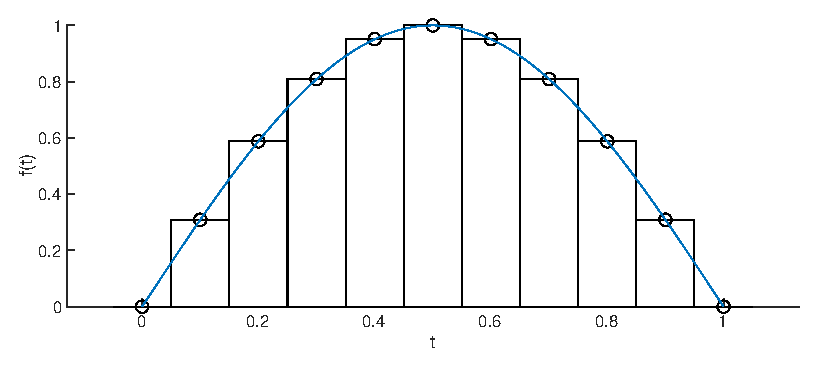
\includegraphics[width=1\textwidth]{figures/quadratureA.eps}
		\caption{Quadrature using the Midpoint Rule}
		\label{fig:quadrature-a}
	\end{figure}
This implementation of a quadrature is called \emph{Midpoint Rule}. 
\\

A more sophisticated way to determine the area of an unbounded integral is to use the Gauss-Hermite Formula

	\begin{equation}
	\int_{-\infty}^{\infty} f(x)e^{-x^2} dx \approx \sum_{i=1}^{n}{w_if(x_i)}
	\end{equation}

where the weights $w_i$ are given as the solution to a linear system of equations and the nodes $x_i$ correspond to the zeros of the n-th Hermite polynomial \citep{seminar:week6}.

\subsection{Dynamic Programming}

A common technique to solve optimization or combinatorial problems is called Dynamic Programming. 
It is based on the idea of dividing problems into smaller subproblems, solving these recursively and caching intermediate results (\textit{memoization}). % Nicht eher "memoRization"?
In his paper "The Theory Of Dynamic Programming" from 1957, Richard Bellman aimed to provide a solution to multi-stage-decision processes. 
He defines a \textit{policy} as "a sequence of decisions" (\cite{bellman:1957}, p.2), and an \textit{optimal policy} as "a policy, which is most advantageous according to some preassigned criterion" (\cite{bellman:1957}, p.2). 
This is reflected in Bellman's Principle of Optimality: "An optimal policy has the property that whatever initial state and initial decisions are, the remaining decisions must constitute an optimal policy with regard to the state resulting from the first decisions" (\cite{bellman:1957}, p.2). 

\subsection{The Bellman Equation}

The so-called "Bellman Equation" answers the question, assuming a given state, what long-term utility can be expected by taking the best possible action now and at each subsequent step - or simply put: "What is the value $V$ of a state $s$?". 

Mathematically, we can express this as  
\begin{equation}
V(s) = \max_{x}(u(s,x) + \beta*V'(s')))
\end{equation}

where $u(s,x)$ is the utility to gain from the control variable (action) $x$ in state $s$ \citep{seminar:week3}. 

So the value of the control variable to be set is the one that maximizes both the utility of the current state plus (recursively) the value $V$ of the next state $s'$ which is discounted by a factor of $\beta$. 


\subsection{Computation of the value function}

In a first step, we want to compute the value function $V$ for each state $s$. 
In order to do so, we need to calculate an auxiliary matrix $aux$ that contains the combined utilities of the farmers and the recreational users. 
Obviously, the $aux$ matrix can only contain a finite, discrete amount of values. In this work, a resolution of $n = 1000$ different water levels and irrigation amounts should suffice. 
Thus we discretize both water level $s$ and irrigation amount $x$ as vectors

	\begin{equation}
s = \left( \begin{array}{c}0\\...\\7\end{array}\right),\hspace{2mm}x = \left( \begin{array}{c}0\\...\\7\end{array}\right)
\end{equation}
% TODO Gibt es hier nicht eine mathematisch schönere Schreibweise um einen Vektor mit 1000 Einträgen darzustellen? (R hoch 1000/ R hoch n)
% TODO das scheint mir nicht so ganz korrekt zu sein. Meint ihr die Dimension?
Note that the maximum reservoir capacity is $7$ and $|s|=|x| = n = 1000$. 

For a combined utility of the farmers and the recreational users  $u(s_i,x_j) = F(x_j) + G(s_i,x_j)$, depending on the water level $s_i$ and the amount of irrigation $x_i$ we get an auxiliary matrix

\begin{dmath}
aux = \left[\begin{array}{ccccc} 
u(s_1, x_1)& \emptyset & \emptyset & ... & \emptyset \\ u(s_2, x_1)& u(s_2, x_2)& \emptyset & ... & \emptyset \\                                               u(s_3, x_1)& ... & u(s_3, x_3)& ... & \emptyset \\                                              ... & ... & ... & ... & \emptyset \\                                              u(s_n, x_1)& ... & ... & ... & u(s_n, x_n)\\                                               \end{array}\right]+\beta*\left[ \begin{array}{ccccc}
V'(s_1') & \emptyset & \emptyset & ... & \emptyset \\                                               V'(s_1') & V'(s_2') & \emptyset & ... & \emptyset \\                                               V'(s_1') & ... & V'(s_3') & ... & \emptyset \\                                              ... & ... & ... & ... & \emptyset \\                                              V'(s_1') & ... & ... & ... & V'(s_n') \\                                               \end{array}\right]
\end{dmath}

where the upper right triangle of this matrix will be empty, as the amount of water, that can be taken from the reservoir must be smaller or equal to the amount of water in the reservoir. 

Here, $V'$ represents the value for $V$ in the previous iteration and will be set to $V'(s'_1) = (0,...0)^T$. Iteratively, we use the bellman equation to calculate a new optimal V: 

\begin{equation}
V(s) = \max_{x}(u(s,x) + \beta*V'(s')))
\end{equation}
\label{eq:value-function}

which equals to finding the column $aux$ that maximizes the expected value over all states.
We repeat this step over and over again until the our value function $V$ converges.
In our case the function converges, if the norm of the difference between $V'$ and $V$ falls below a certain tolerance value \\

% Finally, we want to compute the value of the steady state by using a monte carlo simulation. 

%------------------------------------------------
\newpage
\section{Results}
This chapter will discuss the outcomes and results of the implemented functionality in MATLAB.
The discussion will be started on the basic questions asked by the project description.
Furthermore we made several modifications to the task which will be discussed additionally.
All results will be visualized by plots made within our simulation in MATLAB.
\subsection{Optimal irrigation policy}
When questioning what the optimal irrigation policy is, the first question to be asked is how the aggregated value function of both recreational users and farmers looks like.
The value function as posed in \ref{eq:value-function} contains the maximum possible usage that can be gained by irrigating a specific amount of water under a given water level. 
Figure \origref{fig:value-function} shows the value function calculated for all possible water levels between the allowed boundaries of 0 and 7. 
\begin{figure}[ht]
	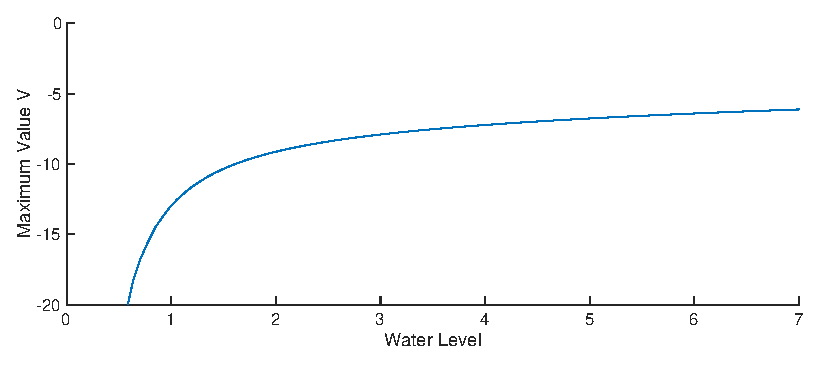
\includegraphics[width=1\textwidth]{figures/value_function.eps}
	\caption{Value Function}
	\label{fig:value-function}
\end{figure}
\newline
Every value along the possible water levels is mapped to an irrigation amount that optimizes the value for all parties in the given situation. Summarizing these values over the range of possible water levels results in a optimal irrigation policy which is shown in \ref{fig:optimal-irrigation-policy}.
The plot shows a rising proposed irrigation amount with rising water level. There are 2 particularities that can be found within the graph:
\begin{itemize}
	\item Due to the effect that a almost empty reservoir has a very low use to recreational users, the optimal irrigation strategy suggests a very low irrigation amount whose gradient increases with increasing water level.
	\item The diminishing margin utility of farmers lead to a decreasing gradient for the proposed irrigation amount with increasing water level.
\end{itemize}
\begin{figure}[ht]
	\includegraphics[width=1\textwidth]{figures/OptimalIrrigationPolicy.eps}
	\caption{Optimal Irrigation Policy}
	\label{fig:optimal-irrigation-policy}
\end{figure}
\newpage
\subsection{Steady State}
In systems theory, a system or a process is in a steady state, if the variables which define the behavior of the system are unchanging in time \citep{gagniuc2017markov}. 
The variable defining the behavior of our system is the water level. 
Because of this, we have to calculate the difference in water level for each period. 
Due to the fact, that our water level highly depends on the randomly distributed rainfalls that fill the reservoir at end of each period, it is not possible to find a steady state in which the water level does not change at all. 
To analyze it nevertheless, we defined our steady state, to be a state, where the mean water level of the last 200 periods did not change more than $1*10^{-7}$ from a period to the next.
A exemplary graph of the mean in every period and the difference to its predecessor is shown in \ref{fig:steadyState}.
Once a period is found, where the mean does not change more than the given value, the mean of that period is defined as steady state water level.
The water level found to be a steady state and the period in which this condition occurs changes from calculation to calculation due to the fact, that the rainfall is still a random distribution.
\begin{figure}[ht]
	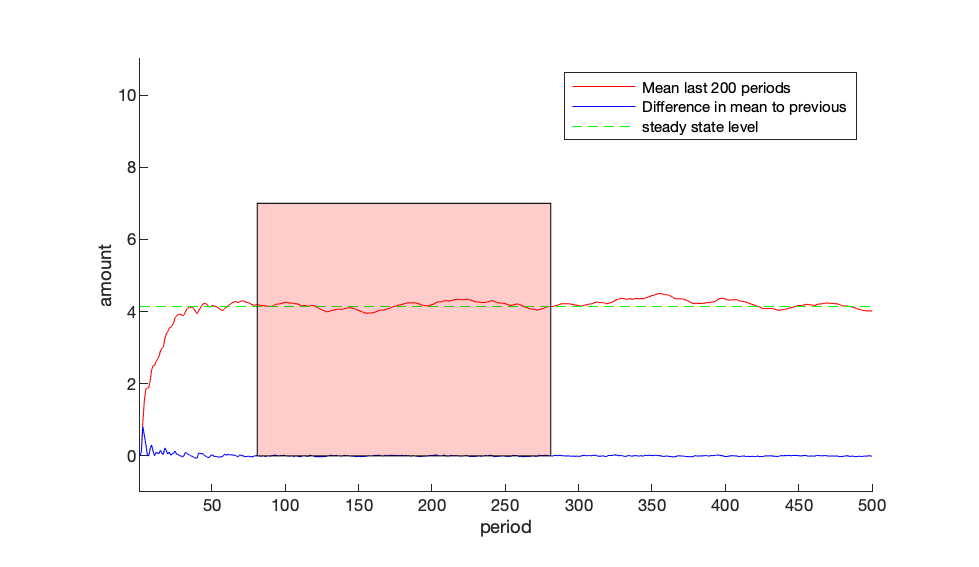
\includegraphics[width=1\textwidth]{figures/steadyState.eps}
	\caption{Exemplary Calculation of the Steady State}
	\label{fig:steadyState}
\end{figure}
\subsection{Steady State Probability}
As mentioned above, the steady state changes from simulation to simulation.
In order to find out, how the steady states are distributed and what the probability of their occurrences are, we did a Monte Carlo simulation.
To do so, we ran our code 1000 times and put the resulting water levels into bins with the size of 0.1 each. % "the forward simulation" instead of "our code"?
We then counted the occurrences, normalized them and calculated the corresponding probability.
The result is put in a histogram and shown in \ref{fig:steadyStateMonteCarlo}.
The highest possibility for a steady state is around 4.2. 
In edge cases one can find steady states as low as 3.5 or as high as 5.2. 
The curve resembles a normal distribution. 

\begin{figure}[ht]
	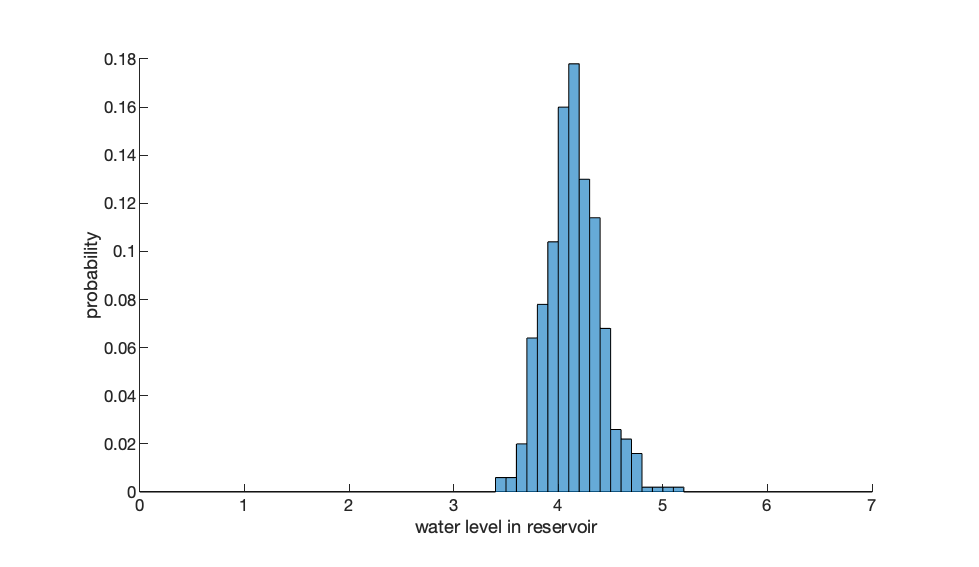
\includegraphics[width=1\textwidth]{figures/steadyStateMonteCarlo.eps}
	\caption{Steady State Probability}
	\label{fig:steadyStateMonteCarlo}
\end{figure}
\subsection{Effect of Changed Discount Factors to Optimal Irrigation Policy}
When altering the discount factor $\beta$ in a range from 0 to 1, the optimal irrigation policy changes.
Looking at small water levels within the reservoir the optimal irrigation amount does not change much depending on the discount factor.
A small $\beta$ ensures that high water levels at the end of one period are only available to a small extent in the next period. % Finde die Formulierung nicht so gut: Sie sind ja weiterhin voll verfügbar, aber eben in Zukunft weniger wert. Bzw das könnte man diskutieren.
This leads to a increasing gap between irrigation amounts over $\beta$ with increasing water level since conserving water does not increase the usage as much.
One can say that a high $\beta$ prefers a long-term policy while a smaller $\beta$ leads to a rather short-term policy.
\begin{figure}[ht]
	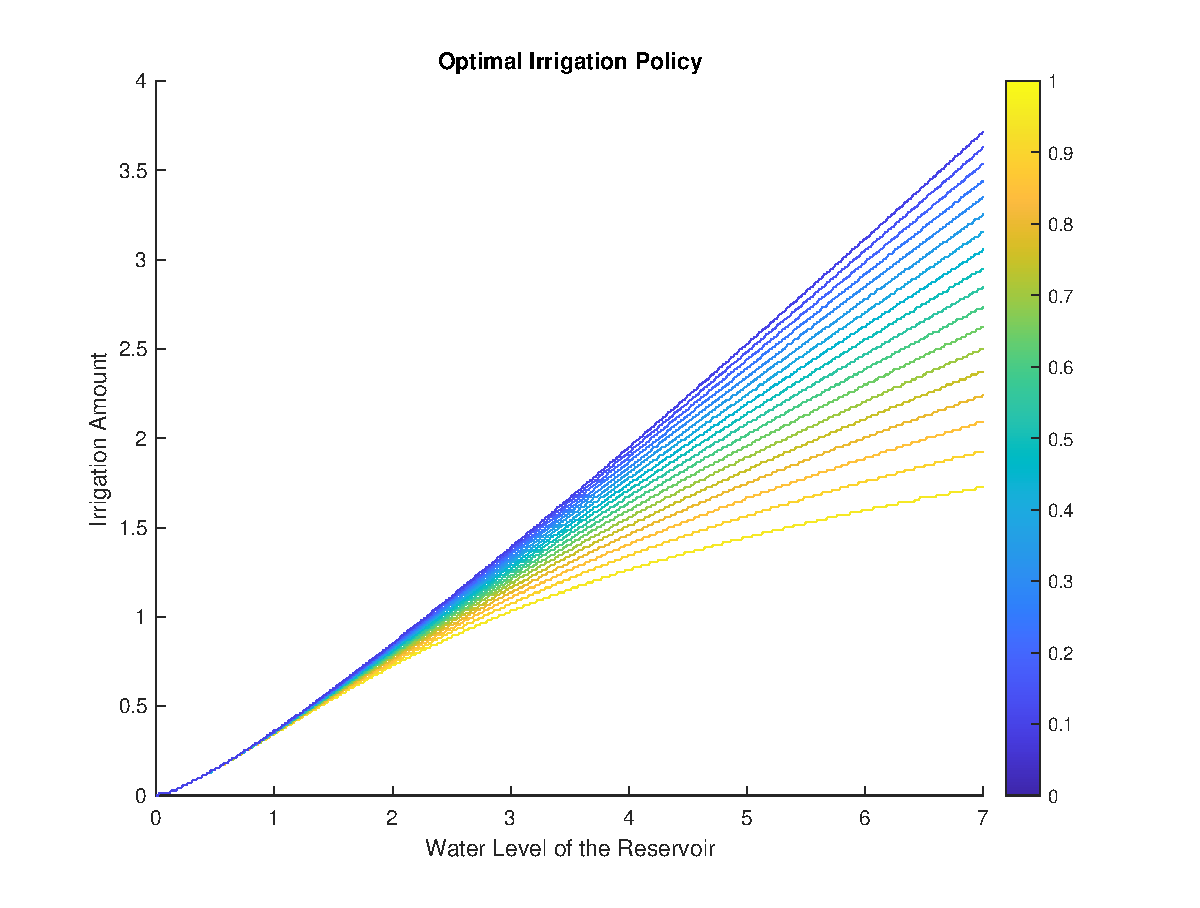
\includegraphics[width=1\textwidth]{figures/optimum-policy-over-beta.eps}
	\caption{Optimal irrigation policy as a function of the discount factor $\beta$}
	\label{fig:optimal-irrigation-beta}
\end{figure}
\newpage
\subsection{Changed Volatility of Rainfalls}
A more volatile rainfall means a rainfall having a higher standard deviation.
Since we want to compare two rainfall distributions of the same mean, the median of the distribution has to be changed.
Using a $\sigma^2=2$ includes a mean of $\mu=-1.5$ in order for the mean to stay the same. 
(See \ref{eq:rainfall} for reference) 
\begin{equation}
	mean = exp(\mu+\frac{\sigma^2}{2}) \label{eq:rainfall}
\end{equation} 
Both distributions are visualized in \ref{fig:rain-distributions}.
\begin{figure}
	\begin{subfigure}{0.5\textwidth}
		\centering
		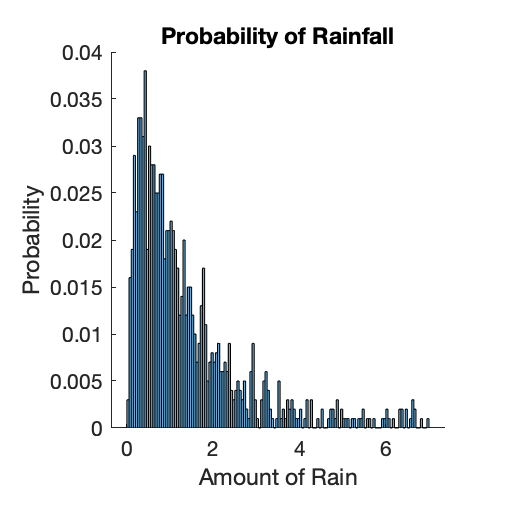
\includegraphics[width=1\textwidth]{figures/rainfall-default.eps}
		\caption{$\mu=0, \sigma=1$}
		\label{fig:rainfall-default}
	\end{subfigure}%
	\begin{subfigure}{.5\textwidth}
		\centering
		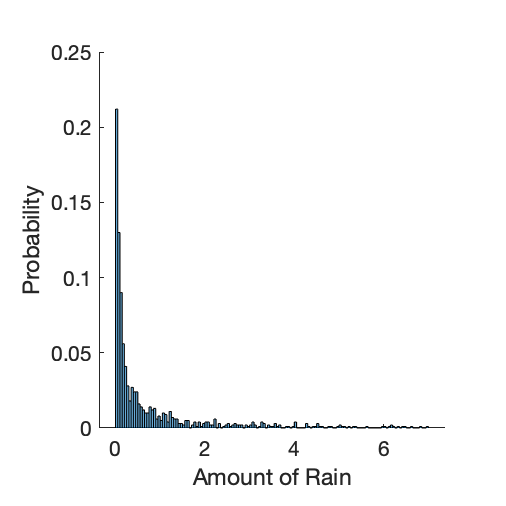
\includegraphics[width=1\textwidth]{figures/rainfall-more-volatile.eps}
		\caption{$\mu=-1.5, \sigma=2$}
		\label{fig:rainfall-changed}
	\end{subfigure}
	\caption{Different Rain Distributions}
	\label{fig:rain-distributions}
\end{figure}
\newpage
\begin{figure}[ht]
	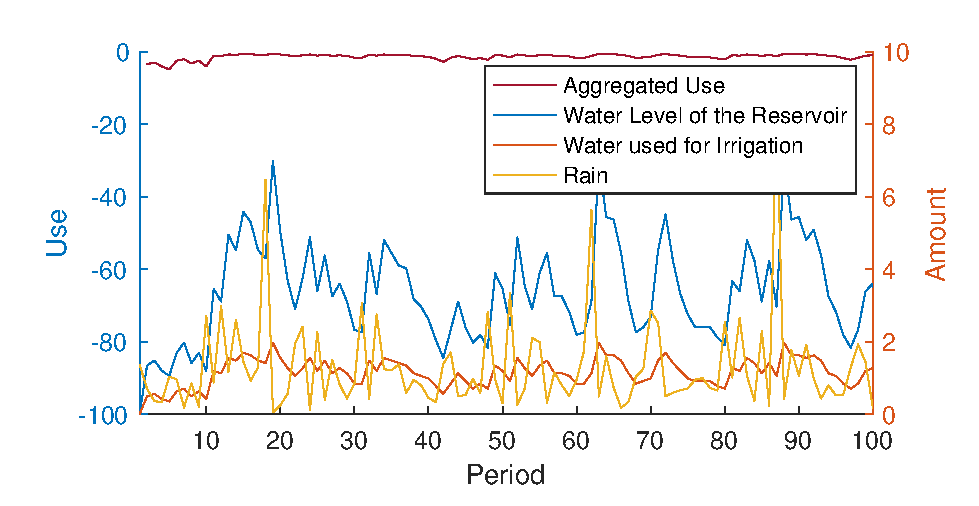
\includegraphics[width=1\textwidth]{figures/aggregated-use-rainfall-default.eps}
	\caption{Aggregated Use for lognormal distributed rainfall $(\mu=0, \sigma=1)$}
	\label{fig:aggregated-use-rainfall-default}
\end{figure}
\begin{figure}[ht]
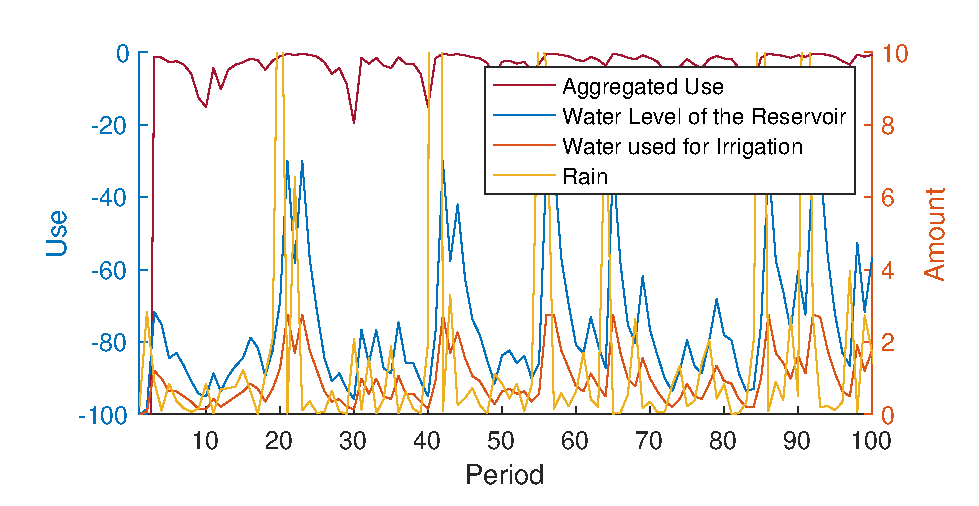
\includegraphics[width=1\textwidth]{figures/aggregated-use-rainfall-more-volatile.eps}
\caption{Aggregated Use for lognormal distributed rainfall $(\mu=-1.5, \sigma=2)$}
\label{fig:aggregated-use-rainfall-more-volatile}
\end{figure}
\ref{fig:aggregated-use-rainfall-default} shows the aggregated use of a lognormal distributed rainfall including the water level, the amount of water used for irrigation in the rain exemplary for 100 periods. \ref{fig:aggregated-use-rainfall-more-volatile} does the same for a changed lognormal distribution parameterized with $\mu=-1.5$ and $\sigma=2$.
When comparing both visualizations, it is noticeable that more volatile rainfall leads to much higher peaks of rain in combination with reduced number of periods with a decent amount of rain. 
As a consequence the water level in the reservoir fluctuates much more leading to periods with almost no water in the reservoir. 
In such periods the farmers use almost no water for irrigation.
The aggregated use of farmers and recreational users drops significantly.
Since the reservoir is capped at a amount of 7, the high peaks of rainfall can not be used to a large extent to fill up the reservoir.
Generally speaking, one can say that a more volatile rain distribution leads to a lower average water level in the reservoir with lower amounts of water to be used for irrigation.
This effect is reflected in the aggregated use as well. 
The use of more volatile rainfall is much lower compared to rainfall parameterized with $\mu=0$ and $\sigma=1$.
Since the mean stays constant within the analyzed comparison, the value function does not change.
\clearpage
\subsection{Using Real Data for Rainfall}
Figure \origref{fig:rainfall-real-data} shows the distribution of rain from a real data set.
Comparing this with \ref{fig:rainfall-default} shows a similar shape of the distribution. 
Since there are only 65 periods within the real data set is not as well distributed as in the lognormal distributed simulation.
\begin{figure}[h]
\begin{subfigure}{0.5\textwidth}
	\centering
	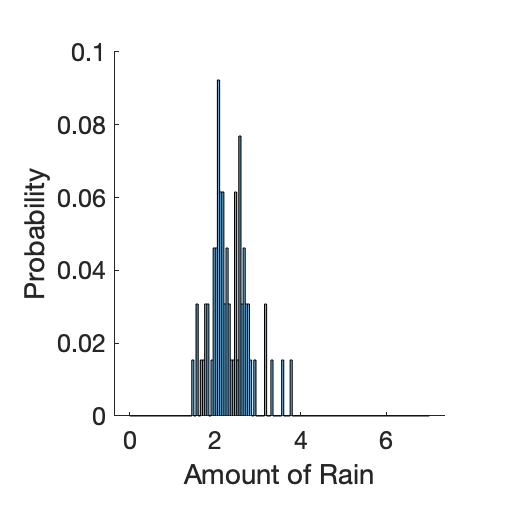
\includegraphics[width=1\textwidth]{figures/rainfall-real-data.eps}
	\caption{Rainfall Distribution from Real Data}
	\label{fig:rainfall-real-data}
\end{subfigure}%
\begin{subfigure}{.5\textwidth}
	\centering
	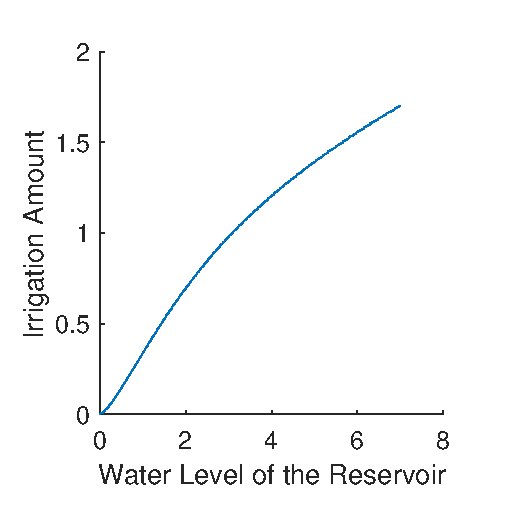
\includegraphics[width=1\textwidth]{figures/optimalIrrigationPolicy-real-data.eps}
	\caption{Optimal Irrigation Policy with Real Data}
	\label{fig:optimalIrrigationPolicy-real-data}
\end{subfigure}
\end{figure}
In the real data set there are no periods with (almost) no rain while in our simulation there are.
As we can learn from our dataset this assumption is not realistic.
Since the amount of rain is scaled down to match our model, there is no comparison between means of the model possible.
Nevertheless one can say that the overall shape of a lognormal distribution is a feasible estimation for rainfall but for estimating whole years as periods the distribution might to be parameterized differently to fit actual rainfalls.
As shown in \ref{fig:optimalIrrigationPolicy-real-data} the changed distribution of rainfalls also has an effect on the optimal irrigation policy since it depends on the expected amount of rain.
Due to the higher expected value of rainfalls the optimal irrigation policy is steeper over the water level compared to the simulated rainfall.

\clearpage	
\newpage

\subsection{Evaporation}
In the following, we want to assess the effect of evaporation on the optimal irrigation policy and the steady state. 
As described in \ref{sec:intro-mod4}, we derive the amount of evaporation over time from other weather related and geographical data. 
The (calculated) evaporation has a low volatility over the years and has value of approximately 1 unit, as \ref{fig:without-vs-with-evaporation} shows. 
Due to the fact that the reservoir has a fixed capacity of 7 units, rainfall that would fill the reservoir above this value is not available for further use. 
When taking evaporation into account, the reservoir never reaches its capacity limits and thus all rainfall will be saved. This leads to an increased volatility of the water level. 
\\


\begin{figure}[h]
\begin{subfigure}{0.5\textwidth}
	\centering
	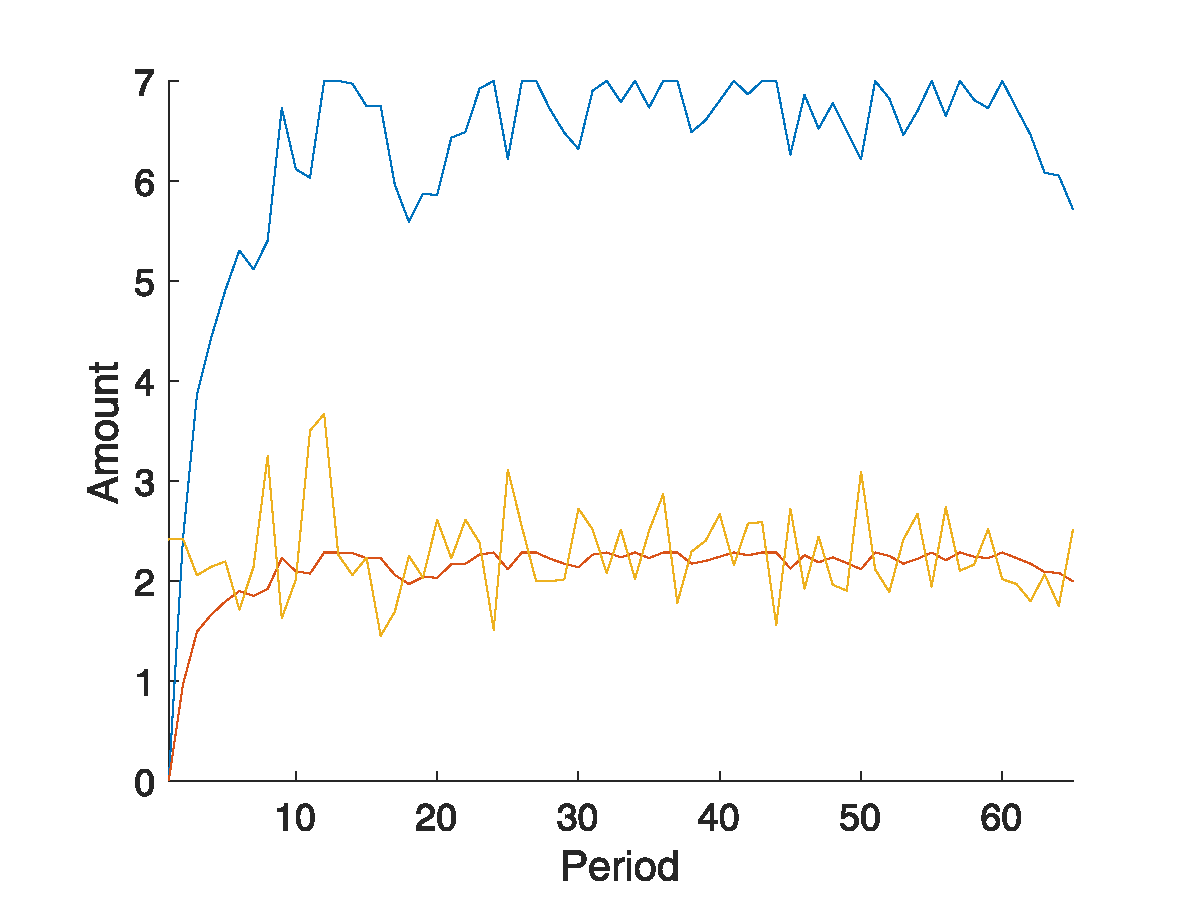
\includegraphics[width=1\textwidth]{figures/results-opt-irrigation-over-time-evap-inactive.eps}
	\caption{Without Evaporation}
	\label{fig:rainfall-real-data}
\end{subfigure}%
\begin{subfigure}{.5\textwidth}
	\centering
	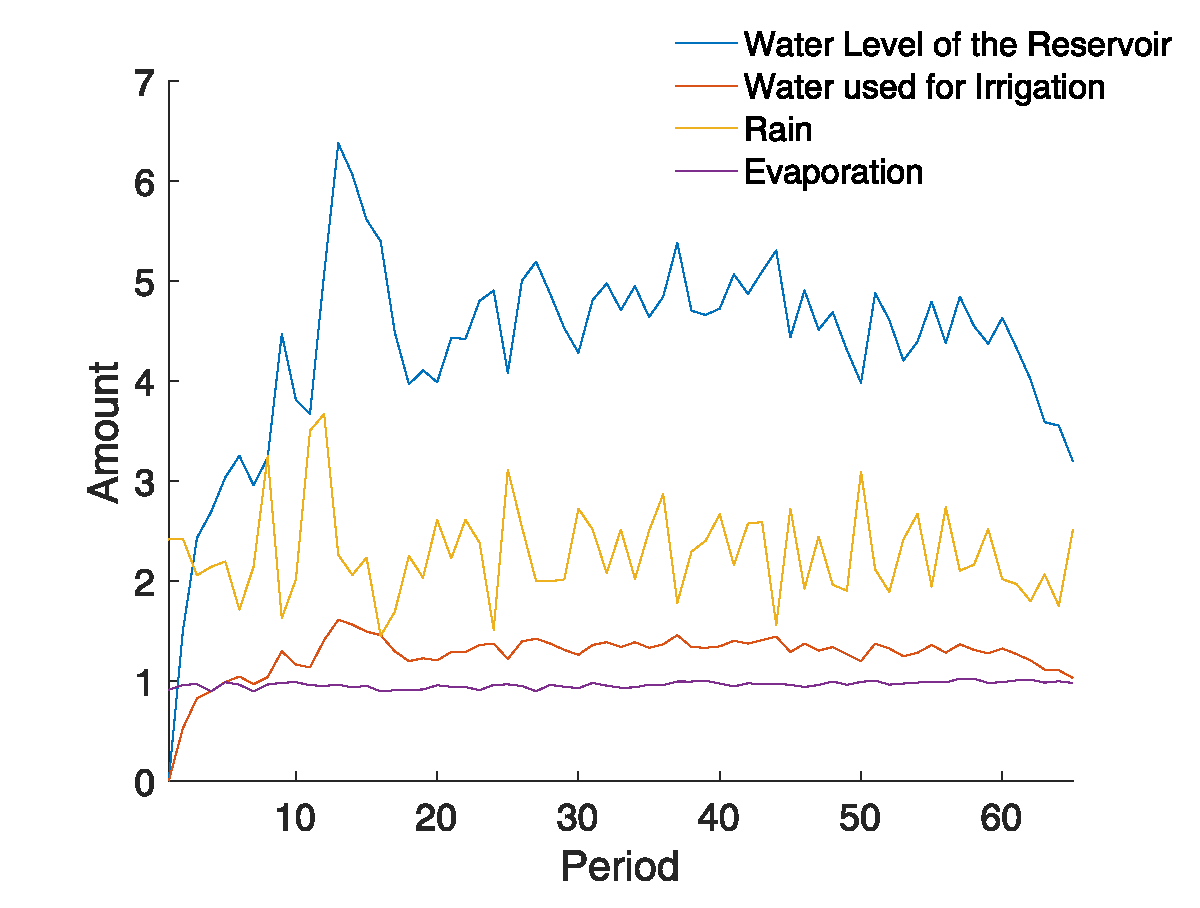
\includegraphics[width=1\textwidth]{figures/results-opt-irrigation-over-time-evap-active.eps}
	\caption{With Evaporation}
	\label{fig:value-function}
\end{subfigure}
\caption{Comparison of water level, irrigation amount, rainfall and evaporation over time using real data}
\label{fig:without-vs-with-evaporation}
\end{figure}

As expected, the average water level is lower with evaporation than without, which in return leads to a lower irrigation the farmers are allowed to receive. \\
In the introduction, we stated that due to climate change, prolonged dry periods will occur. We want to reflect this fact in the simulation by scaling the evaporation rate with different factors. 

%TODO make the figure better
\begin{figure}[ht]
\begin{subfigure}{0.5\textwidth}
	\centering
	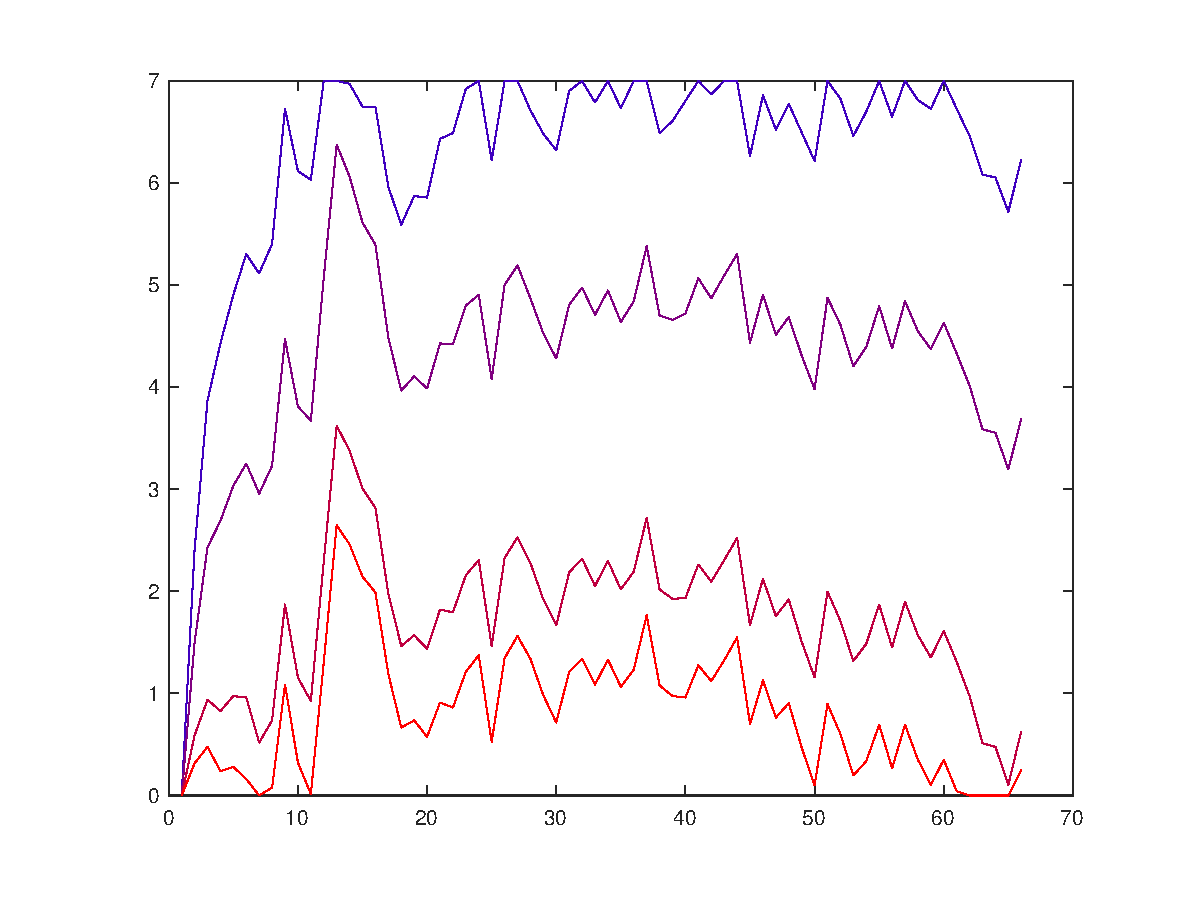
\includegraphics[width=1\textwidth]{figures/results-evap-factors-water-levels.eps}
	\caption{Water Level}
	\label{fig:rainfall-real-data}
\end{subfigure}%
\begin{subfigure}{.5\textwidth}
	\centering
	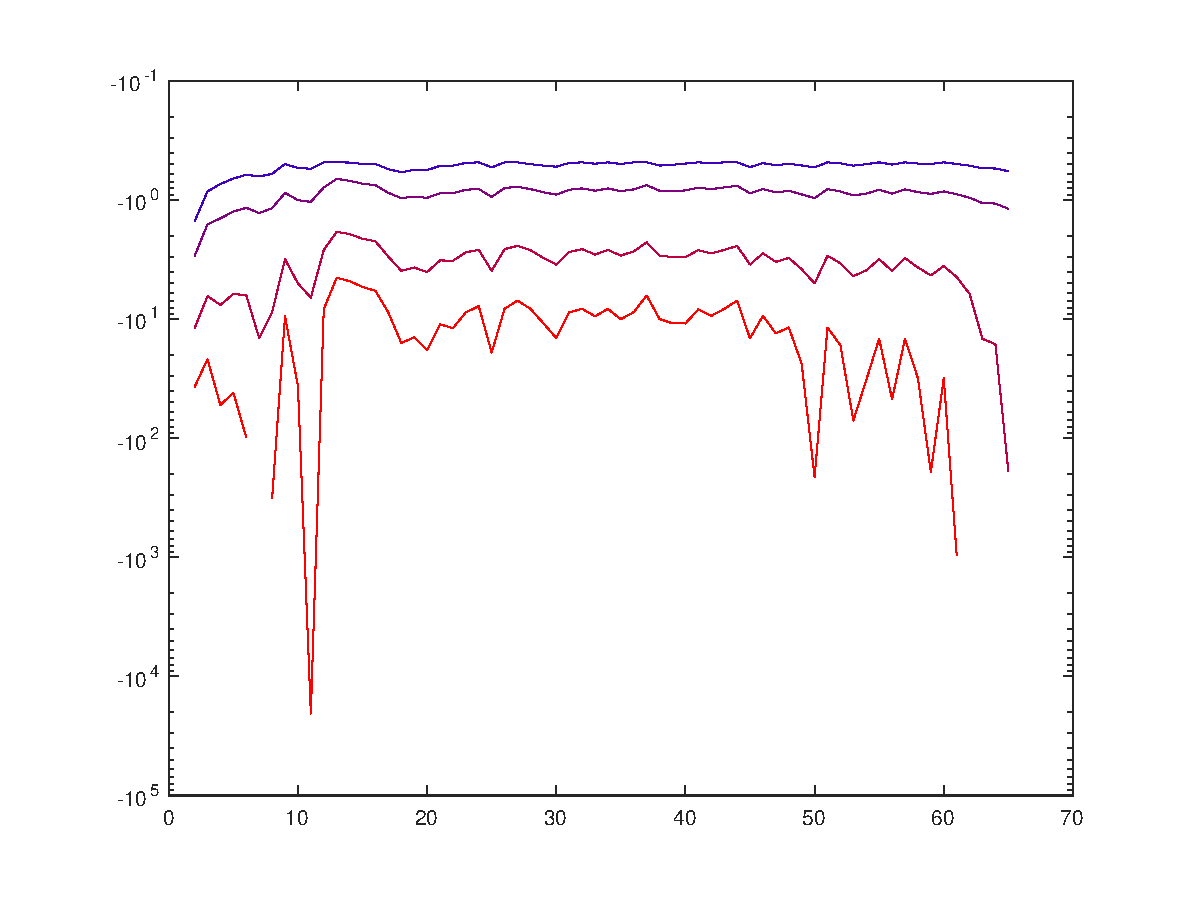
\includegraphics[width=1\textwidth]{figures/results-evap-factors-utilities.eps}
	\caption{Total Utility}
	\label{fig:value-function}
\end{subfigure}
\caption{Water level and log-scaled total utility over time, scaling evaporation with factors $0, 1, 2, 2.3$ (from top to bottom)}
\label{fig:evaporation-factors}
\end{figure}
%\clearpage

\ref{fig:evaporation-factors} shows the total utility and the water level over time, using scaling factors of $0, 1, 2, 2.3$.\footnote{The expected value of the evaporation should not exceed the expected value of the rainfall, as this would make it impossible to calculate the value function. The expected value of the evaporation with a scaling factor of $2.3$ is just below the expected value of the rainfall. } %TODO Fußnote gut so?
We can see that higher amounts of evaporation not only lead to water levels, but also to significantly lower utilities for the recreational users and the farmers. 
Especially when the reservoir completely dries out, the total utility approaches $-\infty$. This happens in periods $7,62,63,64$ and $65$ when applying a factor of $2.3$ to the evaporation. 

%TODO improve this figure
\begin{figure}[h]
	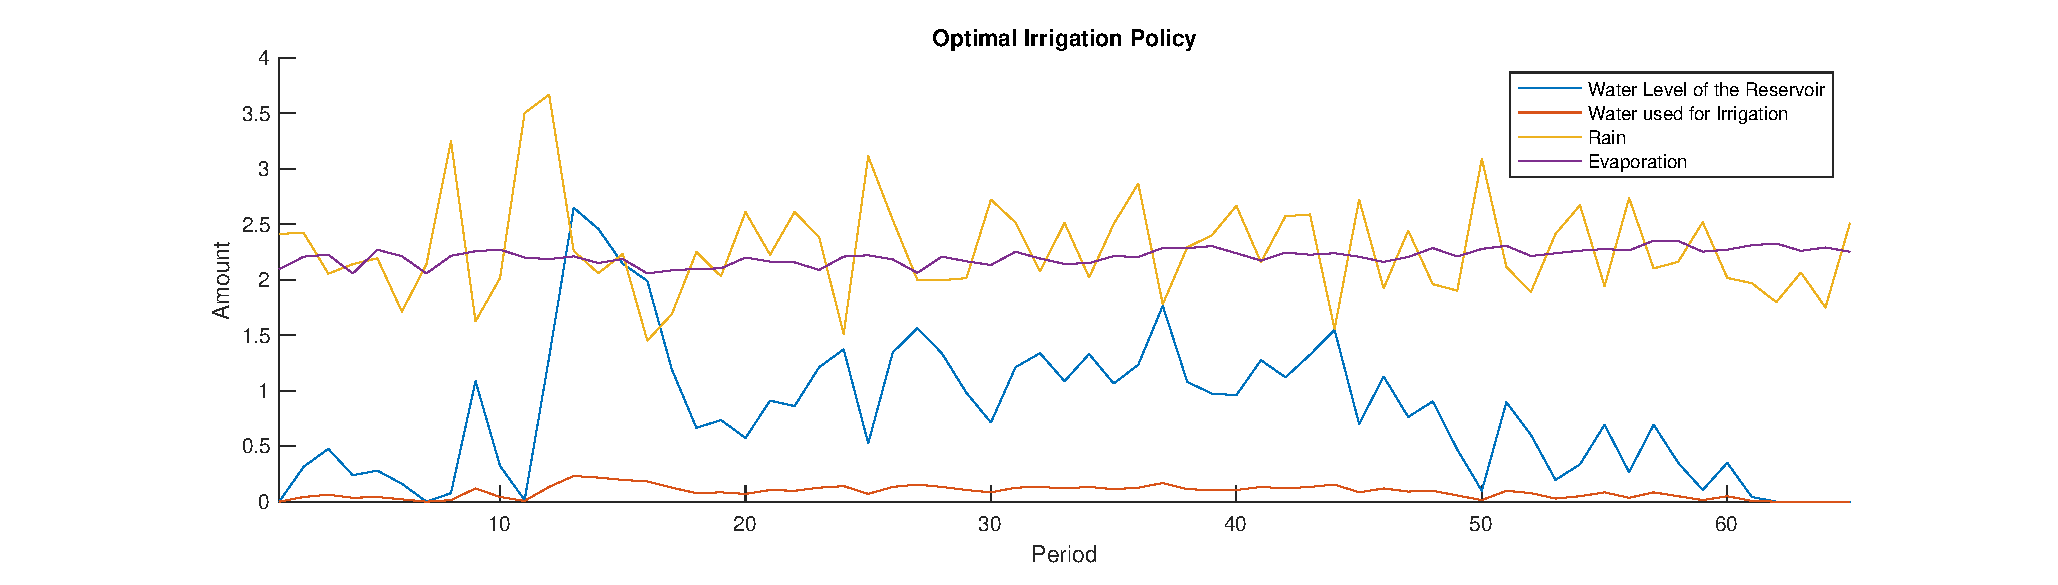
\includegraphics[width=1\textwidth]{figures/results-evap-factor-2.3.eps}
	\caption{Evaporation multiplied by a factor of $2.3$ outweighs the rainfall in certain periods} %TODO 
	\label{fig:evap-factor-2.3}
\end{figure}

The reason for this is found in the utility functions of the farmers and the recreational users. Because of $x\leq s$, we get for $s\to 0 \Rightarrow x\to 0$, and as a consequence 

\begin{equation}
\lim_{s, x\to0}F(x) = \lim_{s,x\to0}-\frac{1}{x} = -\inf
\end{equation}

as well as

\begin{equation}
\lim_{s, x\to0}G(s,x) = \lim_{s,x\to0}-\frac{1}{(s-x)^2} = -\inf
\end{equation}




%TODO den folgenden Absatz rauswerfen?
How then can these utility functions be interpreted in terms of reality? 
An utility value of negative infinity may be reasonable, if an actor has no alternative actions available. 
In this scenario, we could imagine this to be an isolated village, where the only possibility for the farmers to irrigate their fields is to use water from this particular reservoir, and the only way to have food for survive is to make use of their own fields (nothing else to do, no trading for example), assuming that the farmers want to survive. 

\section{Conclusion}
%TODO content
\clearpage
\printbibliography

\newpage






%----------------------------------------------------------------------------------------
%	STATUTORY DECLARATION IN LIEU OF AN OATH
%----------------------------------------------------------------------------------------
\pagestyle{empty} 
\begingroup
\begin{center}
	\large
	\textbf{Eidesstattliche Versicherung}
\end{center}

\vspace{0.3cm}

\begin{tabular}{@{}p{8cm}p{5.8cm}}
	\underline{\hspace{6cm}} & \underline{\hspace{5.8cm}} \\
	\vspace{0.02cm}Name, Vorname & \vspace{0.02cm}Matrikelnummer \\
	&\\
	\underline{\hspace{6cm}} & \underline{\hspace{5.8cm}} \\
	\vspace{0.02cm}Name, Vorname & \vspace{0.02cm}Matrikelnummer \\
	&\\
	\underline{\hspace{6cm}} & \underline{\hspace{5.8cm}} \\
	\vspace{0.02cm}Name, Vorname & \vspace{0.02cm}Matrikelnummer \\
\end{tabular}
\vspace{0.3cm}

Ich versichere hiermit an Eides Statt, dass ich die vorliegende Arbeit mit dem Titel

\begin{center}
	{\makeatletter{\emph{{\@title}}}\makeatother}
\end{center}

selbständig und ohne unzulässige fremde Hilfe erbracht habe. Ich habe keine anderen als die angegebenen Quellen und Hilfsmittel benutzt. Für den Fall, dass die Arbeit zusätzlich auf einem Datenträger eingereicht wird, erkläre ich, dass die schriftliche und die elektronische Form vollständig übereinstimmen. Die Arbeit hat in gleicher oder ähnlicher Form noch keiner Prüfungsbehörde vorgelegen.

\vspace{0.6cm}

\begin{tabular}{@{}p{8cm}p{5.8cm}}
	\underline{\smash{Aachen, den \hspace{4cm}}} & \underline{\hspace{5.8cm}}\\
	Ort, Datum & Unterschrift \\
	&\\
	\underline{\smash{Aachen, den \hspace{4cm}}} & \underline{\hspace{5.8cm}}\\
	Ort, Datum & Unterschrift \\
	&\\
	\underline{\smash{Aachen, den \hspace{4cm}}} & \underline{\hspace{5.8cm}}\\
	Ort, Datum & Unterschrift \\
\end{tabular}

\vspace{0.6cm}

\begin{small}
	\textbf{Belehrung:}\\
	Wer vorsätzlich gegen eine die Täuschung über Prüfungsleistungen betreffende Regelung einer Hochschulprüfungsordnung verstößt, handelt ordnungswidrig. Die Ordnungswidrigkeit kann mit einer Geldbuße bis zu 50 000 Euro geahndet werden. Zuständige Verwaltungsbehörde für die Verfolgung und Ahndung von Ordnungswidrigkeiten ist die Kanzlerin oder der Kanzler der RWTH Aachen. Im Falle eines mehrfachen oder sonstigen schwerwiegenden Täuschungsversuches kann der Prüfling zudem exmatrikuliert werden (§ 63 Abs. 5 HG NRW).
	
	\textbf{§ 156 StGB: Falsche Versicherung an Eides Statt}\\
	Wer vor einer zur Abnahme einer Versicherung an Eides Statt zuständigen Behörde eine solche Versicherung falsch abgibt oder unter Berufung auf eine solche Versicherung falsch aussagt, wird mit Freiheitsstrafe bis zu drei Jahren oder mit Geldstrafe bestraft.
	
	\textbf{§ 161 StGB: Fahrlässiger Falscheid; fahrlässige falsche Versicherung an Eides Statt}\\
	(1) Wenn eine der in den §§ 154 bis 156 bezeichneten Handlungen aus Fahrlässigkeit begangen worden ist, so tritt Freiheitsstrafe bis zu einem Jahr oder Geldstrafe ein.\\
	(2) Straflosigkeit tritt ein, wenn der Täter die falsche Angabe rechtzeitig berichtigt. Die Vorschriften des § 158 Abs. 2 und 3 gelten entsprechend
\end{small}

\vspace{0.6cm}

Die vorstehende Belehrung habe ich zur Kenntnis genommen:

\vspace{0.6cm}
\begin{tabular}{@{}p{8cm}p{5.8cm}}
	\underline{\smash{Aachen, den \hspace{4cm}}} & \underline{\hspace{5.8cm}}\\
	Ort, Datum & Unterschrift \\
	&\\
	\underline{\smash{Aachen, den \hspace{4cm}}} & \underline{\hspace{5.8cm}}\\
	Ort, Datum & Unterschrift \\
	&\\
	\underline{\smash{Aachen, den \hspace{4cm}}} & \underline{\hspace{5.8cm}}\\
	Ort, Datum & Unterschrift \\
\end{tabular}

\endgroup
\clearpage
	
\end{document}
